% =========================================================
% dokument.tex -- Taylorovy rady: vyukovy material
% Seminar IVT, 3. rocnik gymnazia
%
% Kompilace: XeLaTeX
%   latexmk -xelatex -cd dokument/dokument.tex
% =========================================================

\documentclass[12pt, a4paper]{article}

% --- Čeština ---
\usepackage{polyglossia}
\setmainlanguage{czech}
\usepackage{fontspec}

% --- Okraje ---
\usepackage[top=20mm, bottom=20mm, left=22mm, right=22mm]{geometry}

% --- Matematika ---
\usepackage{amsmath}
\usepackage{amssymb}

% --- Čísla s desetinnou čárkou ---
\usepackage{siunitx}
\sisetup{
    output-decimal-marker = {,},
    group-separator       = {\,},
}

% --- Grafika ---
\usepackage{graphicx}
\usepackage{float}
\usepackage{caption}
\usepackage{tikz}

% --- Tabulky ---
\usepackage{booktabs}
\usepackage{array}

% --- Rámečky ---
\usepackage{mdframed}

% --- Zdrojový kód ---
\usepackage{xcolor}
\usepackage{listings}

\definecolor{codebg}{RGB}{245,245,245}
\definecolor{codegreen}{RGB}{0,120,0}
\definecolor{codepurple}{RGB}{120,0,140}
\definecolor{codeblue}{RGB}{0,0,180}
\definecolor{codegray}{RGB}{120,120,120}

\lstdefinestyle{python}{
    language=Python,
    backgroundcolor=\color{codebg},
    basicstyle=\ttfamily\small,
    keywordstyle=\color{codeblue}\bfseries,
    commentstyle=\color{codegreen}\itshape,
    stringstyle=\color{codepurple},
    numberstyle=\tiny\color{codegray},
    numbers=left,
    numbersep=8pt,
    breaklines=true,
    showstringspaces=false,
    frame=single,
    framerule=0.4pt,
    rulecolor=\color{gray!50},
    tabsize=4,
    captionpos=b,
}
\lstset{style=python}

% --- České uvozovky ---
\usepackage{csquotes}
\newcommand{\uv}[1]{\enquote{#1}}

% --- Bibliografie ---
\usepackage[backend=biber, style=iso-numeric, sorting=none]{biblatex}
\addbibresource{../literatura.bib}

% --- Hyperlinks (vždy poslední) ---
\usepackage{hyperref}
\hypersetup{colorlinks=true, linkcolor=blue!60!black, urlcolor=blue!60!black}

% =========================================================
% Rámečky
% =========================================================
\newmdenv[
    linewidth=1pt,
    linecolor=blue!60!black,
    backgroundcolor=blue!4,
    innertopmargin=8pt, innerbottommargin=8pt,
    innerleftmargin=10pt, innerrightmargin=10pt,
    skipabove=\baselineskip, skipbelow=\baselineskip,
]{defbox}

\newmdenv[
    linewidth=1pt,
    linecolor=orange!70!black,
    backgroundcolor=orange!5,
    innertopmargin=8pt, innerbottommargin=8pt,
    innerleftmargin=10pt, innerrightmargin=10pt,
    skipabove=\baselineskip, skipbelow=\baselineskip,
]{notebox}

% =========================================================
% Titulní informace
% =========================================================
\title{Taylorovy řady\\[0.4em]
       \large Jak kalkulačka počítá goniometrické funkce}
\date{2025}

% =========================================================
\begin{document}
% =========================================================

\maketitle
\tableofcontents
\newpage

% =========================================================
\section{Motivace: co dělá kalkulačka, když stisknete sin?}
% =========================================================

Když na kalkulačce stisknete klávesy \texttt{3}, \texttt{0},
\texttt{sin}, dostanete výsledek \num{0.5}.
Ale jak ho kalkulačka spočítala?
Neexistuje jednoduchý vzorec pro sinus, který by se dal přímo vyhodnotit.
Kalkulačka musí použít některý z~aproximačních algoritmů.

V~praxi se používají tyto hlavní metody:

\begin{itemize}
    \item \textbf{Maclaurinovy řady} (Taylorovy v~bodě $x = 0$) ---
          nekonečný polynom, který přesně reprezentuje hladké funkce.
          Intuitivní a výchozí bod pro pochopení.
    \item \textbf{Čebyševovy polynomy} (minimax aproximace) ---
          polynom, který minimalizuje maximální odchylku na daném
          intervalu. Přesnější než Taylor pro stejný stupeň.
    \item \textbf{CORDIC} (Coordinate Rotation Digital Computer) ---
          algoritmus používající jen bitové posuvy a sčítání.
          Vhodný pro jednoduché čipky bez násobiček~\cite{volder1959}.
    \item \textbf{Tabulky s~interpolací} ---
          kompromis mezi pamětí a rychlostí; kalkulačky 70.~let.
\end{itemize}

\begin{notebox}
\textbf{Proč studujeme Taylorovy řady?}
Konvergují pomaleji než moderní metody a pro velká $x$ jsou nepřesné.
Ale jsou \emph{intuitivní} a jsou \emph{výchozím bodem} pro pochopení
aproximačních algoritmů. Čebyšev, CORDIC a další vycházejí ze stejné
myšlenky: funkci lze lokálně přiblížit polynomem.
\end{notebox}

% =========================================================
\section{Co je Taylorova řada?}
% =========================================================

\begin{defbox}
\textbf{Taylorova řada} funkce $f$ v~bodě $a$ je nekonečný polynom:
\[
    f(x)
    = f(a) + f'(a)(x-a)
    + \frac{f''(a)}{2!}(x-a)^2
    + \frac{f'''(a)}{3!}(x-a)^3
    + \cdots
    = \sum_{n=0}^{\infty} \frac{f^{(n)}(a)}{n!}(x-a)^n
\]
\emph{Značky $f'(a)$, $f''(a)$, \ldots{} jsou derivace v~bodě $a$
--- pojmy z~vyšší matematiky, ke kterým se dostanete v~budoucích
hodinách. Vzorci stačí věřit; obrázek níže ukáže, co znamená.}

Pro $a = 0$ se řada nazývá \textbf{Maclaurinova}.
\end{defbox}

Intuice: každá hladká funkce lze lokálně přiblížit polynomem.
Čím více členů vezmeme, tím přesnější aproximace.
Nekonečný součet dává přesnou hodnotu (tam, kde řada konverguje).

\subsection{Vizuální demonstrace}

Na následujícím obrázku je znázorněno, jak polynomy stupně 1, 3, 5, 7
přibližují $\sin(x)$ na intervalu $\langle -\pi, \pi \rangle$.
Čím vyšší stupeň, tím lepší shoda.

\begin{figure}[H]
\centering
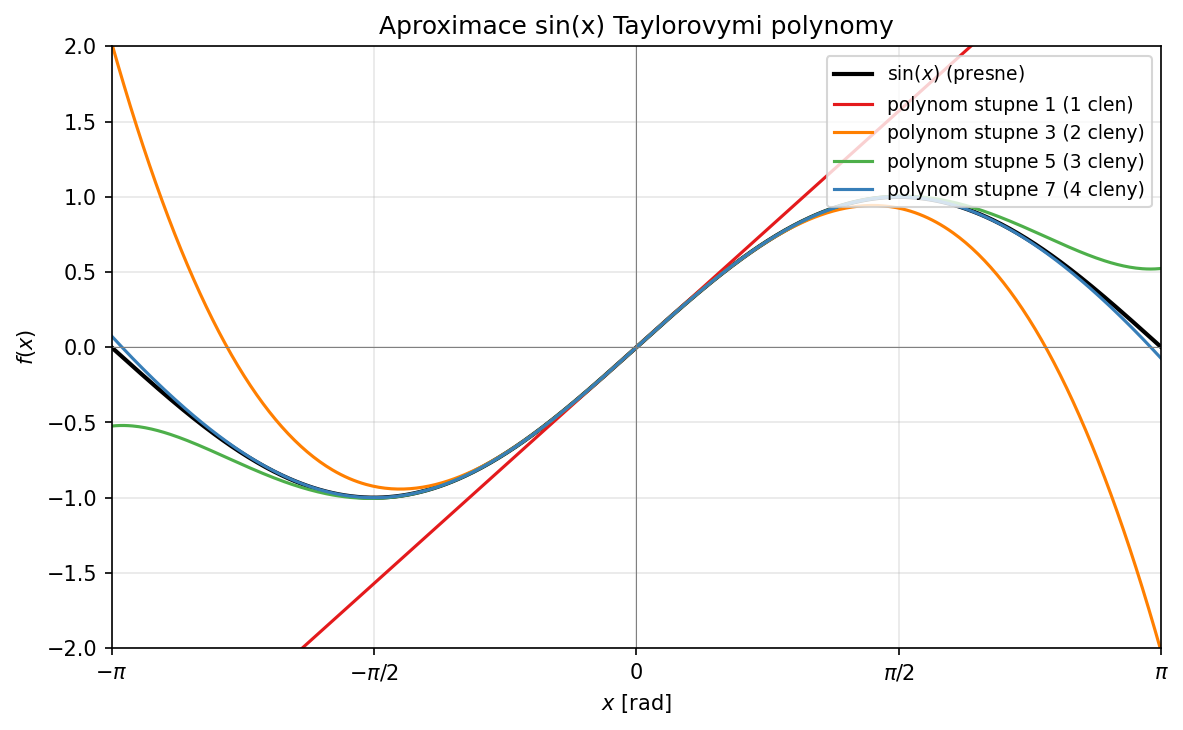
\includegraphics[width=0.85\textwidth]{../python/output/sin_aproximace.png}
\caption{Aproximace $\sin(x)$ Taylorovými polynomy různého stupně.
         Černá čára je přesná hodnota; barevné čáry jsou polynomy
         se 1, 2, 3 a 4 členy řady (stupně 1, 3, 5, 7).}
\label{fig:sin_aproximace}
\end{figure}

\begin{notebox}
\textbf{Derivace?}
V~obrázku vidíte: polynom prvního stupně (přímka $y = x$) je
v~bodě $x_0 = 0$ tečna ke křivce.
Přidáním členu $-x^3/6$ získáme lepší shodu.
Každý další člen opravuje chybu toho předchozího.
Koeficienty včetně $n! = 1 \cdot 2 \cdots n$ ve jmenovateli
pocházejí z~derivací, které zatím nemusíme znát ---
stačí nám věřit, že vzorec funguje.
\end{notebox}

% =========================================================
\section{Sinus a kosinus}
% =========================================================

\subsection{Vzorce}

\begin{defbox}
\textbf{Maclaurinova řada pro $\sin(x)$:}
\[
    \sin(x)
    = x - \frac{x^3}{3!} + \frac{x^5}{5!} - \frac{x^7}{7!} + \cdots
    = \sum_{k=0}^{\infty} \frac{(-1)^k\, x^{2k+1}}{(2k+1)!}
\]

\textbf{Maclaurinova řada pro $\cos(x)$:}
\[
    \cos(x)
    = 1 - \frac{x^2}{2!} + \frac{x^4}{4!} - \frac{x^6}{6!} + \cdots
    = \sum_{k=0}^{\infty} \frac{(-1)^k\, x^{2k}}{(2k)!}
\]
\end{defbox}

\begin{notebox}
\textbf{Pozor: $x$ musí být v~radiánech!}
Převod: $x_\mathrm{rad} = x_\circ \cdot \frac{\pi}{180}$.
Například $30^\circ = \frac{\pi}{6} \approx \num{0.5236}~\mathrm{rad}$.
\end{notebox}

\subsection{Ruční výpočet: $\sin(30^\circ)$}

Převod: $x = 30^\circ = \frac{\pi}{6}$.
Přesná hodnota: $\sin(\pi/6) = 0{,}5$.

Výpočet s~prvními třemi členy:

\[
    \sin\!\left(\frac{\pi}{6}\right)
    \approx
    \underbrace{\frac{\pi}{6}}_{\approx\,0{,}5236}
    -
    \underbrace{\frac{(\pi/6)^3}{3!}}_{\approx\,0{,}0239}
    +
    \underbrace{\frac{(\pi/6)^5}{5!}}_{\approx\,0{,}0003}
    \approx
    \num{0.5000}
\]

Chyba při 3 členech: $|0{,}500002 - 0{,}5| \approx 2 \times 10^{-6}$. Po 5 členech
je chyba pod $10^{-10}$.

\subsection{Konvergence sinu}

\begin{figure}[H]
\centering
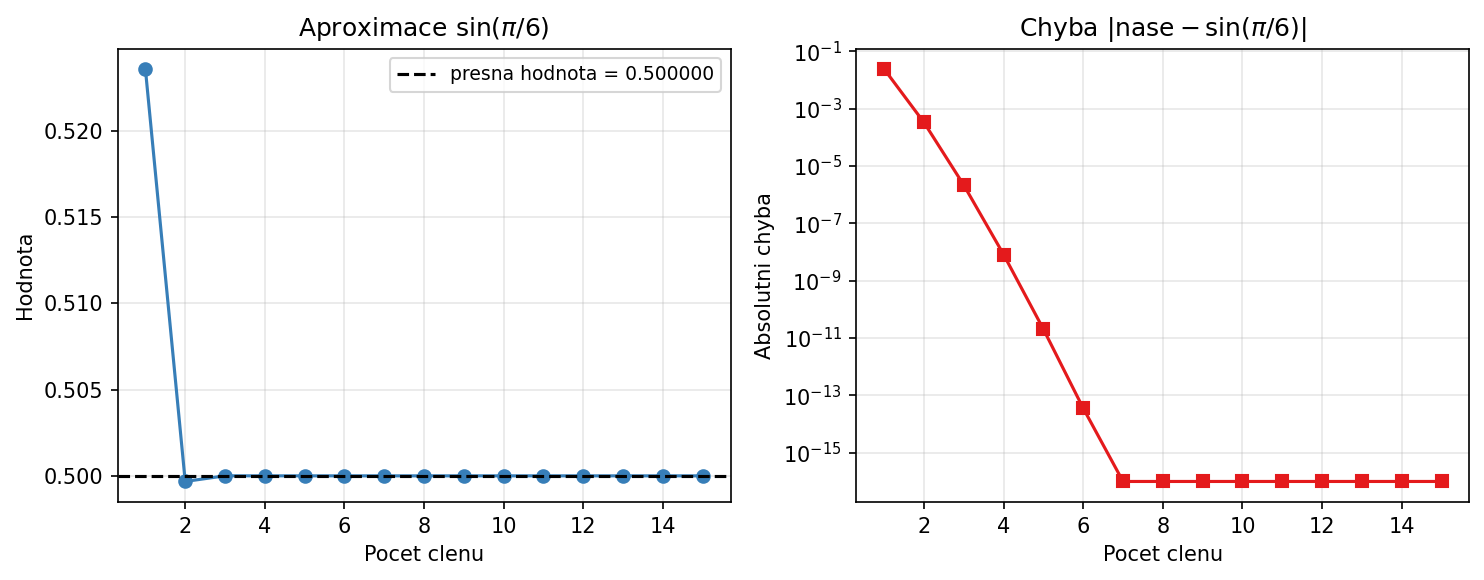
\includegraphics[width=0.85\textwidth]{../python/output/sin_konvergence.png}
\caption{Konvergence $\sin(\pi/6)$ pro rostoucí počet členů řady.
         Vlevo hodnota aproximace, vpravo absolutní chyba (logaritmická osa).}
\label{fig:sin_konvergence}
\end{figure}

\subsection{Konvergence kosinu}

Analogicky pro $\cos(\pi/3) = 0{,}5$
(přesná hodnota; argument $\pi/3 \approx \num{1.047}$~rad je větší než $\pi/6$,
takže řada konverguje o~trochu pomaleji):

\begin{center}
\begin{tabular}{@{}rrl@{}}
\toprule
Členů & Hodnota          & Chyba        \\ \midrule
1     & $\num{1.0000000}$ & $\num{5.0e-1}$ \\
2     & $\num{0.4516886}$ & $\num{4.8e-2}$ \\
3     & $\num{0.5017962}$ & $\num{1.8e-3}$ \\
5     & $\num{0.5000004}$ & $\num{4.0e-7}$ \\
7     & $\num{0.5000000}$ & $< 10^{-12}$ \\ \bottomrule
\end{tabular}
\end{center}

\begin{figure}[H]
\centering
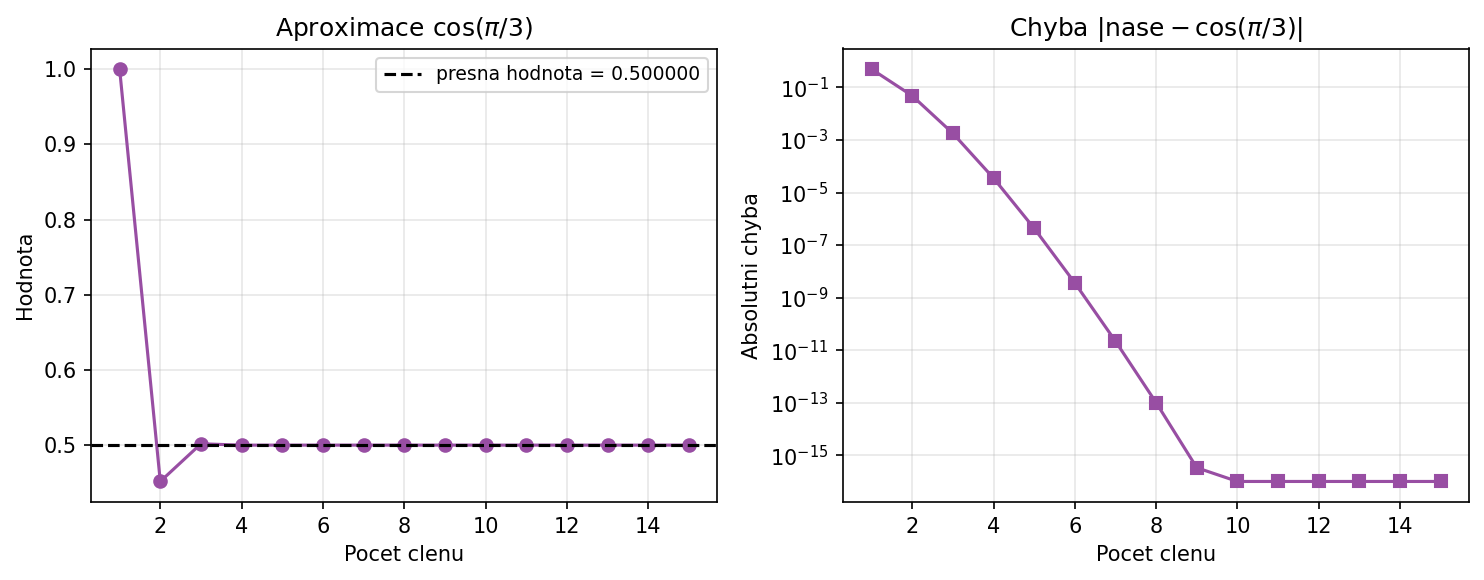
\includegraphics[width=0.85\textwidth]{../python/output/cos_konvergence.png}
\caption{Konvergence $\cos(\pi/3)$ pro rostoucí počet členů řady.
         Vlevo hodnota aproximace, vpravo absolutní chyba (logaritmická osa).}
\label{fig:cos_konvergence}
\end{figure}

% =========================================================
\section{Odmocnina --- Newtonova iterace}
% =========================================================

\subsection{Historický kontext: 3700 let stará metoda}

Zhruba v~roce 1700 př.~n.~l.\ zapsal neznámý babylonský písař
na hliněnou tabulku YBC~7289 výpočet $\sqrt{2}$ na šest platných
číslic: ${\approx}\,1{,}41421$
(v~sexagesimální soustavě: $1;\, 24,\, 51,\, 10$).
Algoritmus, který použil, je přesně ten, který budeme implementovat.

Metoda se později ztratila a~byla nezávisle znovuobjevena několikrát:
v~antice ji popsal Heron z~Alexandrie (1.~stol.~n.~l.),
a~v~17.~století ji Isaac Newton zformuloval jako speciální případ
obecného algoritmu pro řešení rovnic (dnes \emph{Newtonova metoda}).
Proto název --- přes veškerou spravedlnost je \uv{newtonská}
jen nejmladší z~mnoha jmen této myšlenky.

\subsection{Myšlenka: obklíčení správné hodnoty}

Chceme vypočítat $\sqrt{a}$.
Zvolme nějaký počáteční odhad $x_0 > 0$ (např. $x_0 = a$).

Klíčem jsou tato jednoduchá pozorování:

\begin{itemize}
    \item Pokud $x_n > \sqrt{a}$, pak $\dfrac{a}{x_n} < \sqrt{a}$
          (protože $x_n \cdot \dfrac{a}{x_n} = a = \sqrt{a} \cdot \sqrt{a}$).
    \item Pokud $x_n < \sqrt{a}$, pak naopak $\dfrac{a}{x_n} > \sqrt{a}$.
\end{itemize}

Jinými slovy: $x_n$ a $\dfrac{a}{x_n}$ \emph{obklíčují} $\sqrt{a}$
z~obou stran. Jejich průměr
\[
    x_{n+1} = \frac{x_n + \dfrac{a}{x_n}}{2}
\]
leží blíže ke správné hodnotě než který z~nich sám.
Opakováním se interval obklíčení rychle zužuje.

\begin{defbox}
\textbf{Newtonova (babylonská) iterace pro $\sqrt{a}$:}
\[
    x_0 = a, \qquad
    x_{n+1} = \frac{x_n + \dfrac{a}{x_n}}{2}
\]
Používá jen $+$, $\times$ a $/$. Žádné mocniny ani faktoriály.
\end{defbox}

\begin{notebox}
\textbf{Nerovnost průměrů (bonusová poznámka).}
Z~nerovnosti aritmetického a~geometrického průměru plyne:
\[
    \frac{x_n + \dfrac{a}{x_n}}{2}
    \;\geq\; \sqrt{x_n \cdot \frac{a}{x_n}}
    = \sqrt{a}.
\]
To znamená, že každý další odhad $x_{n+1}$ je \emph{vždy větší nebo roven}
$\sqrt{a}$ --- iteraci nikdy nepodstřelíme.
Po prvním kroku tedy pracujeme jen s~nadodhadem,
který se monotónně snižuje k~přesné hodnotě.
\end{notebox}

\subsection{Odkud se bere vzorec? (Pro zvídavé)}

Možná jste si všimli, že vzorec vypadá jako průměr $x_n$ a $a/x_n$.
Kde se ale vzal?

Chceme najít $x$ takové, že $x^2 = a$, neboli řešit rovnici
$f(x) = x^2 - a = 0$.
Newton měl nápad: v~bodě $x_n$ nahraď $f$ přímkou (tečnou),
zjisti, kde ta přímka protíná \emph{vodorovnou čáru $y = a$},
a~proveď to jako nový odhad. Situaci ukazuje obrázek~\ref{fig:tikz_newton}.

\begin{figure}[H]
\centering
\begin{tikzpicture}[x=3.2cm, y=0.72cm, >=latex, font=\small]
  % === Osy ===
  \draw[->] (1.15,0) -- (2.22,0) node[right] {$x$};
  \draw[->] (1.15,0) -- (1.15,4.7) node[above] {$y$};
  \foreach \yy in {1,2,3,4}
    \draw (1.15,\yy) -- (1.12,\yy) node[left] {\yy};
  % === Parabola y = x^2 ===
  \draw[domain=1.19:2.08, smooth, very thick, blue!70!black, samples=60]
    plot (\x, {\x*\x});
  \node[right=3pt, blue!70!black] at (2.08,{2.08*2.08}) {$y=x^2$};
  % === Cilova cara y = 2 ===
  \draw[gray!70, dashed, thick] (1.15,2) -- (2.15,2)
    node[right, gray!80!black] {$y = a = 2$};
  % === Krok 1: x_0 = 2 -> x_1 = 1.5 ===
  \draw[red!25, dashed] (2,0) -- (2,4);
  \node[below, red!80!black] at (2,0) {$x_0=2$};
  \filldraw[red] (2,4) circle (2.2pt);
  \node[above right=-1pt, red] at (2,4) {$(x_0,\,x_0^2)$};
  \draw[red, very thick] (2,4) -- (1.5,2);
  % === Krok 2: x_1 = 1.5 -> x_2 = 1.4167 ===
  \draw[orange!35, dashed] (1.5,0) -- (1.5,2.25);
  \node[below, orange!80!black] at (1.5,0) {$x_1=1{,}5$};
  \filldraw[orange!80!black] (1.5,2.25) circle (2.2pt);
  \node[above right=-1pt, orange!80!black] at (1.5,2.25) {$(x_1,\,x_1^2)$};
  \draw[orange!80!black, very thick] (1.5,2.25) -- (1.4167,2);
  % === x_2 ≈ √2 ===
  \filldraw[green!60!black] (1.4167,2) circle (2.2pt);
  \node[above left=-1pt, green!60!black] at (1.4167,2) {$x_2\approx\sqrt{2}$};
\end{tikzpicture}
\caption{Geometrie Newtonovy iterace pro $a=2$.
         Tečna k~parabolě $y=x^2$ v~bodě $(x_n,\,x_n^2)$
         protíná čáru $y=2$ v~novém odhadu $x_{n+1}$.
         Červeně: krok $x_0\to x_1$; oranžově: $x_1\to x_2$.}
\label{fig:tikz_newton}
\end{figure}

Chceme najít $x$ takové, že $x^2 = a$, neboli řešit rovnici
$f(x) = x^2 - a = 0$.
Newton měl nápad: v~bodě $x_n$ nahraď $f$ přímkou (tečnou),
zjisti, kde ta přímka protíná osu $x$, a~proveď to jako nový odhad.

Bez použití derivací (které tečnu formálně definují) to můžeme zapsat
algebraicky: tečna k~parabole $y = x^2$ v~bodě $(x_n, x_n^2)$
má směrnici $2x_n$ a rovnici $y = x_n^2 + 2x_n(x - x_n)$.
Položíme $y = a$ a vyřešíme $x$:
\[
    a = x_n^2 + 2x_n(x - x_n)
    \;\Longrightarrow\;
    x = \frac{x_n^2 + a}{2x_n}
    = \frac{x_n}{2} + \frac{a}{2x_n}
    = \frac{x_n + a/x_n}{2}.
\]
Dostali jsme přesně náš vzorec. Newtonova metoda je tedy geometricky:
\uv{najdi, kde tečna protíná osu, a zopakuj}.

\subsection{Konvergence je kvadratická}

Počet správných číslic se přibližně zdvojuje při každé iteraci.
Například pro $\sqrt{2}$:

\begin{table}[H]
\centering
\caption{Ruční průchod Newtonovou iterací pro $\sqrt{2}$.
         Správná hodnota: $\num{1.41421356}$.}
\label{tab:sqrt2}
\begin{tabular}{@{}rll@{}}
\toprule
Iterace & $x_n$             & Chyba               \\ \midrule
0       & $2{,}00000000$    & $\num{5.86e-1}$     \\
1       & $1{,}50000000$    & $\num{8.58e-2}$     \\
2       & $1{,}41666667$    & $\num{2.45e-3}$     \\
3       & $1{,}41421569$    & $\num{2.12e-6}$     \\
4       & $1{,}41421356$    & $\num{1.59e-12}$    \\
5       & $1{,}41421356$    & $< 10^{-15}$        \\ \bottomrule
\end{tabular}
\end{table}

\begin{figure}[H]
\centering
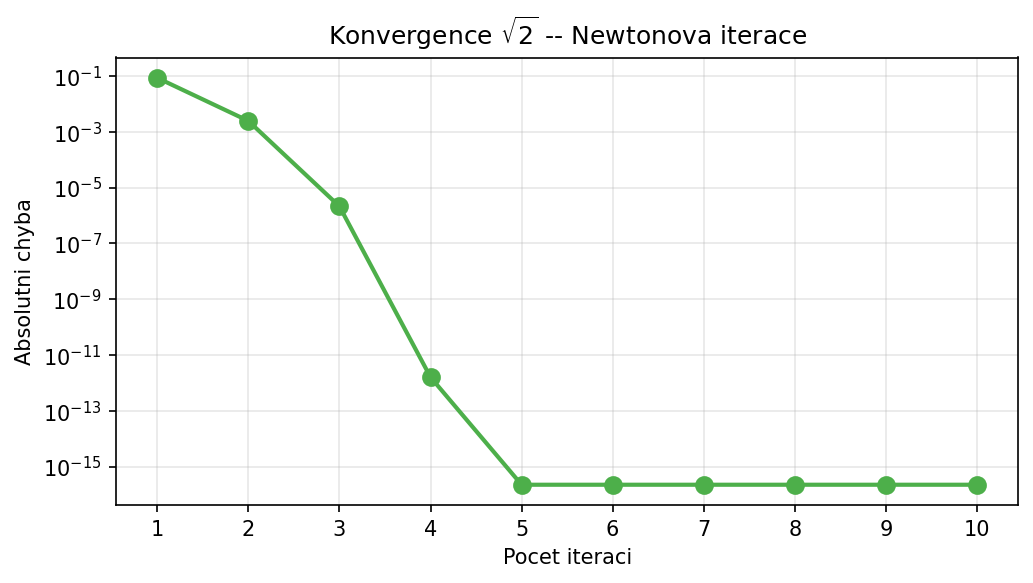
\includegraphics[width=0.75\textwidth]{../python/output/sqrt_konvergence.png}
\caption{Absolutní chyba Newtonovy iterace pro $\sqrt{2}$
         (logaritmická osa). Strmost odpovídá kvadratické konvergenci.}
\label{fig:sqrt_konvergence}
\end{figure}

\begin{notebox}
\textbf{Když je počáteční odhad špatný?}
Volba $x_0 = a$ funguje pro většinu vstupů, ale pro velká $a$
může být pomalejší. Lepší odhad (například $x_0 = 1$) sníží počet
potřebných iterací. Moderní procesory používají tabulku prvního
přiblížení a pak jen 1--2 Newtonovy kroky.
\end{notebox}

% =========================================================
\section{Implementace v~Pythonu}
% =========================================================

\subsection{Implementované funkce}

\begin{lstlisting}[caption={Taylorova řada pro $\sin(x)$.}]
def faktorial(n):
    vysledek = 1
    for i in range(2, n + 1):
        vysledek *= i
    return vysledek

def sin_taylor(x, n_terms=10):
    soucet = 0.0
    for k in range(n_terms):
        exponent = 2 * k + 1
        clen = ((-1) ** k) * (x ** exponent) / faktorial(exponent)
        soucet += clen
    return soucet
\end{lstlisting}

\begin{lstlisting}[caption={Newtonova iterace pro $\sqrt{a}$.}]
def sqrt_newton(a, n_iter=10):
    if a == 0:
        return 0.0
    x = a                    # pocatecni odhad
    for _ in range(n_iter):
        x = (x + a / x) / 2
    return x
\end{lstlisting}

\subsection{Tabulka chyb}

Spuštění \texttt{python python/taylor.py} vytiskne tabulku absolutních
chyb pro různý počet členů a iterací. Ukázka výstupu pro $\sin(\pi/6)$:

\begin{center}
\begin{tabular}{@{}rrl@{}}
\toprule
Členů & Hodnota          & Chyba        \\ \midrule
1     & $\num{0.5235988}$ & $\num{2.4e-2}$ \\
2     & $\num{0.4996742}$ & $\num{3.3e-4}$ \\
3     & $\num{0.5000021}$ & $\num{2.1e-6}$ \\
5     & $\num{0.5000000}$ & $\num{8.8e-11}$ \\
7     & $\num{0.5000000}$ & $< 10^{-15}$ \\ \bottomrule
\end{tabular}
\end{center}

% =========================================================
\section{Co dál? Od Taylora k~Čebyševovi}
% =========================================================

Taylorova řada má jednu slabinu: pro velká $x$ (např. $x = 100$)
konverguje velmi pomalu. Moderní kalkulačky proto nejdříve provedou
\textbf{redukci oboru} (angl.\ \emph{range reduction}): přivedou $x$ do malého
intervalu (např. $[0, \pi/2]$) pomocí vztahu $\sin(x + 2\pi) = \sin(x)$,
a~teprve pak aproximují.

Na intervalu $[0, \pi/2]$ pak používají místo Taylorova polynomu
\textbf{Čebyševův polynom}: namísto toho, aby byl přesný v~$x = 0$
(jako Taylor), minimalizuje maximální chybu na celém intervalu.
Výsledek je přesnější při stejném počtu koeficientů.

Další téma k~prozkoumání: CORDIC~\cite{volder1959} ---
výpočet goniometrických funkcí jen pomocí posunů bitů a sčítání,
bez jakéhokoli násobení.

% =========================================================
\printbibliography[title={Literatura}]

% =========================================================

\end{document}
